\documentclass{beamer}

\usepackage{array}
\usepackage{booktabs}

\newcolumntype{M}[1]{>{\centering\arraybackslash}m{#1}}
\newcolumntype{N}{@{}m{0pt}@{}}
\newcolumntype{C}{>{$\displaystyle}c<{$}}



\usetheme{default}
\usecolortheme{rose}
\usepackage{hyperref}
\newcommand{\ignore}[1]{}
\newcommand{\pr}{\mathbb{P}}
\newcommand{\E}{\mathbb{E}}
\newcommand{\var}{\text{var}}
\newcommand{\sd}{\text{sd}}
\newcommand{\h}{\widehat}
\newcommand{\TS}{\textit{T}}
\newcommand{\ts}{\textit{t}}


\setbeamerfont{alerted text}{series=\itshape}
\addtobeamertemplate{navigation symbols}{}{%
    \usebeamerfont{footline}%
    \usebeamercolor[fg]{footline}%
    \hspace{1em}%
    \insertframenumber/\inserttotalframenumber
}

\title{Review}

% A subtitle is optional and this may be deleted
\subtitle{STAT-UB.0001 Statistics for Business Control}

\author{Ningshan Zhang}
% - Give the names in the same order as the appear in the paper.
% - Use the \inst{?} command only if the authors have different
%   affiliation.

\institute[New York University] % (optional, but mostly needed)
{
  IOMS Department\\
  nzhang@stern.nyu.edu
  \let\thefootnote\relax\footnotetext{\tiny{*  Office Hours: Wed \& Fri 10:00 - 11:30 AM, KMC 8-174}}
}
\date{Aug 7, 2018}
\AtBeginSubsection[]
{
  \begin{frame}<beamer>{Outline}
    \tableofcontents[currentsection,currentsubsection]
  \end{frame}
}

% Let's get started
\begin{document}

%-------------------
\begin{frame}
  \titlepage
\end{frame}

\begin{frame}{Final Exam}
\begin{itemize}
    \item Aug 9, 10:00 - 12:00 AM, Tisch UC19.
    \item Open book and notes. No cellphone or laptop.
    \item Bring a calculator (make sure it cake take square root). 
    \item Covers all the topics; focuses on the second half.
\end{itemize}
\end{frame}


%-------------------
\begin{frame}{Populations vs Samples}
    ``Statistics is using a \alert{sample} to make a statement about a \alert{population}.''
    \vspace{\stretch{0.2}}

        \begin{itemize}
            \item Population: The set of items or individuals that we are interested in studying and drawing conclusions about. 
                \vspace{\stretch{0.2}}
            \item Sample: A subset of items or individuals from the population. 
        \begin{itemize}
            \item Unbiased sample: every member of the population has an equal chance of being included in the sample.
        \end{itemize}
        \end{itemize}
\end{frame}

%-------------------
\begin{frame}{Descriptive Statistics}
    Descriptive Statistics: types of statements.
    \begin{itemize}
        \item Center of the distribution: mean, median.
        \item Spread of the distribution: range, standard deviation.
        \item Shape of the distribution: histogram, boxplot.
    \end{itemize}
\end{frame}

%-------------------
\begin{frame}{Center of the Distribution: Mean vs Median}
\begin{itemize}
\item Mean: the average of the observations:
$$\bar x = \dfrac{1}{n} \sum_{i=1}^n x_i
=\dfrac{1}{n} \left(x_1+x_2 + \dots+x_n\right). $$
\item Median: the middle value in a \alert{sorted} dataset. 
\begin{itemize}
\item  When n is odd, take ``true'' middle value.
\item When n is even, take the average of the two middle values.
\end{itemize}
\item Skewness
    \begin{itemize}
\item Positive/right skew:   mean - median $>0$ , mean is to the right of the median. 
\item Negative/left skew:   mean - median $<0$, mean is to the left of the median. 
\end {itemize}
\end{itemize}
\end{frame}

%-------------------
\begin{frame}{Spread of the Distribution}
\begin{itemize}
\item Range:
    \[
        \max(\{x_1,\cdots,x_n\}) - \min(\{x_1,\cdots,x_n\})
    \]
\item Variance ($s^2$) and standard deviation ($s$):
    \begin{align*}
        s^2 &=\frac{1}{n-1}\sum_{i=1}^n (x_i-\bar x)^2 \\
        s &=\sqrt{s^2}
    \end{align*}

\end{itemize}
\end{frame}

%-------------------
\begin{frame}{Probability: Terminology}
\begin{itemize}
\item Random experiment: the process of observation leading to an outcome that cannot be predicted with certainty.
\item Sample point: a possible outcome of an experiment. 
\item Sample space of experiments: the set of all sample points, denoted by $\Omega$, or $S$.
\item Event: a set of sample points. 
\end{itemize}

Example: flip a coin; roll a 6-sided dice.
\end{frame}

%-------------------
\begin{frame}{Probability}
    \begin{itemize}
        \item Given a sample space, $\Omega=\{e_1,e_2,\cdots,e_n\}$. A probability 
$\pr$  is a function with two properties: 
\begin{align*}
    \pr(e_i)\geq0, \quad \pr(e_1)+ .. + \pr(e_n)=1.
\end{align*}

\item Probability of an event: If $A=\{e_1,\dots,e_m\}$, then
 $$\pr(A)=\pr(e_1) + \dots + \pr (e_m).$$

\item Interpretations of probability: long-run relative frequency; when an  experiment is repeated $n$  times ($n$ is large),
$$\pr(A) \approx (\text{no. of times }A\text{ occured})/n.$$

    \end{itemize}
\end{frame}

%-------------------
\begin{frame}{Compound Events: Union and Intersections}
$A$ and $B$ are two events.
\begin{itemize}
\item Union ($A \cup B$, ``$A$ or $B$''): event $A$ or event $B$ occurs, or both occur. 
\item Intersection ( $A \cap B$, ``$A$ and $B$''): event A and event B both occur.
\begin{center}
\begin{figure}\caption{Left: $A\cap B$. Right: $A\cup B$}
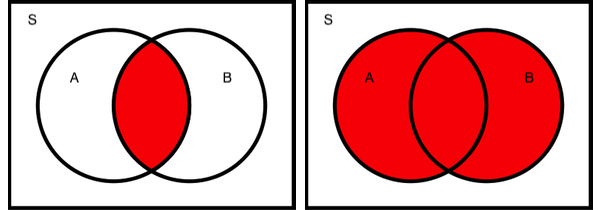
\includegraphics[width=0.6\textwidth]{figures/venn-intersection-union}
\end{figure}\end{center}
\item Mutually exclusive events: $A$ and $B$  cannot occur together, $ \pr(A\cap B)=0$.
\end{itemize}


\end{frame}

%-------------------
\begin{frame}{Conditional Probability and Independence}
    \begin{itemize}
        \item Conditional probability $\pr(A \mid B)$:  the probability of event $A$, given that event $B$ occurred. It is formally defined as 
$$\pr(A\mid B) = \frac{\pr(A \cap B)}{\pr(B)}.$$
\item Statistical independence: A and B are independent events if the occurrence of A does not affect the probability that B occurs:
$$\pr(A \mid B)=\pr(A) \iff\pr(B \mid A)=\pr(B)$$
\end{itemize}
\end{frame}


%-------------------
\begin{frame}{Rules for Computing with Probability}
    \begin{itemize}
        \item Additive rule: 
            \begin{align*}
                \pr(A\cup B) & = \pr(A)+\pr(B) - \pr(A\cap B). \\
                \pr(A\cup B) &= \pr(A)+\pr(B). \tag{\small only when A and B are ME}
            \end{align*}
        \item Complement rule: 
            $$ \pr(A^c) = 1 - \pr(A).$$
        \item Multiplicative rule:
            \begin{align*}
                \pr(A \cap B) &= \pr(B) \pr(A\mid B) = \pr(A)\pr(B \mid A). \\
                \pr(A \cap B) &= \pr(A) \pr(B) \tag{\small only when A and B are independent}
            \end{align*}
    \end{itemize}
\end{frame}

%-------------------
\begin{frame}{Bayes' Rule: relates $\pr(A\mid B)$ to $\pr(B | A)$}
    Given $k$ mutually exclusive events $B_1,B_2,\dots,B_k$ such that $\pr(B_1) + \pr(B_2) + \dots + \pr(B_k)=1$, then
    \begin{align*}
        \pr(B_i \mid A) & = \frac{\pr(A \cap  B_i) }{\pr(A)}\\
        & =
        \frac{\pr(A\mid B_i) \pr(B_i)}
        {\pr(A\mid B_1)\pr(B_1) + \dots + \pr(A\mid B_k) \pr(B_k)}
    \end{align*}

    \begin{itemize}
    \item Bayes' rule can be derived from additive rule and multiplicative rule.
    \end{itemize}
\end{frame}


%-------------------
\begin{frame}{Counting Rules}
When all sample points are equally likely,
$$\pr(A)=\frac{\text{no. of sample points in } A}{\text{no. of sample points in } \Omega}.$$

\begin{itemize}
    \item Permutations rule: The number of ways to arrange $k$ out of $n$ objects is 
    $$P(n,k) = n (n-1) \cdots (n-k+1)=\frac{n!}{(n-k)!}.$$
    \item Combinations rule: 
        Number of ways to pick \alert{unordered} $k$  out of $n$  objects is
        \begin{align*}
            C(n,k)&=\frac{\text{ no. of ways to pick \alert{ordered} $k$ objects out of $n$  }}
            {\text{no. of ways to order $k$ objects}}\\
            & = \frac{P(n,k)}{k!} = \frac{n!}{k!(n-k)!}
        \end{align*}
\end{itemize}
\end{frame}

%-------------------
\begin{frame}{Random Variable}

\begin{itemize}
    \item Random Variable: A variable whose value depends uniquely on the outcome of a random experiment. 
    \item Properties of a discrete random variable $X$:
        \begin{itemize}
            \item Probability Distribution Function (PDF): $$ p(x) = \pr(X=x).$$
            \item Expected value/mean/expectation ($\mu$, $\mu_X$):
                $$\E(X)=\sum_{x} x\cdot p(x)$$
            \item Variance ($\sigma^2$, $\sigma_X^2$) and standard deviation ($\sigma$, $\sigma_X$):
                $$ \var(X) = \sum_x (x-\mu)^2 p(x),\quad \sd(X)=\sqrt{\var(X)} $$
        \end{itemize}
\end{itemize}
\end{frame}

\begin{frame}{Continuous Random Variables}
X is a continuous random variable. 
\vspace{\stretch{0.1}}
\begin{itemize}
\item The probability of $X$ taking any \alert{individual value} is $0$.
$$\pr(X=x)=0, \text{ for any value of }x.$$
\item The probability of $X$ \alert{within a range of values} is defined by probability density function (pdf):
\begin{figure}
    \caption{The pdf and the area under the curve.}
    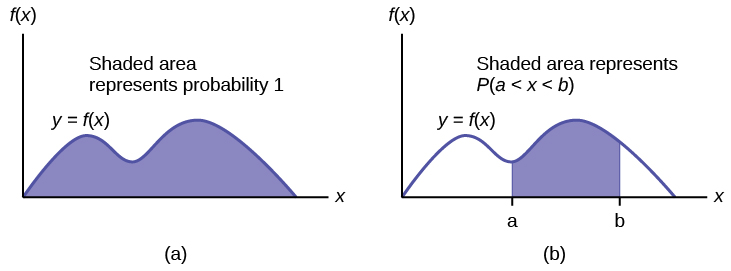
\includegraphics[width=0.8\textwidth]{figures/pdf.jpg}
\end{figure}

\end{itemize}
\end{frame}


%-------------------
\begin{frame}{Properties of Expected Value}
\begin{enumerate}
\item (Aaffine transformation) Let $a,b$ be two constants, and let $X$ be a random variable. Then,
$$ \E(aX+b) = a \E(X) + b$$
\vspace{-0.4cm}
\item (Sum) Let $X$ and $Y$ be two random variables. Then,
$$ \E(X+Y) = \E(X)+\E(Y)$$
\end{enumerate}
Applications:
$$
\E(-X)=-\E(X),\quad \var(aX) = a^2 \var(X)
$$
\end{frame}


%-------------------
\begin{frame}{The Binomial Distribution}
Binomial experiment:
\begin{itemize}
\item It consists of a fixed number \alert{$n$} of statistically independent trials;
\item each trial has the same probability of success \alert{$p$};
\item we want to count the number of successes.  
\end{itemize}

\vspace{\stretch{0.2}}
Let $X$ = the number of successes. Then X is a \alert{binomial random variable} that has \alert{binomial distribution}, 
written as $X \sim B(n,p)$. The PDF, mean and standard deviation are:
    \begin{align*}
        \pr(X=k) &= \binom{n}{k} p^k (1-p)^{n-k},\\
        \E(X)&=np, \quad \var(X) = np(1-p).
\end{align*}
\end{frame}

\begin{frame}{The Poisson Distribution}
Let $X$ = the number of events that occur in a fixed interval of time, space, etc.  Assume that
\begin{itemize}
\item Events occur with a known constant rate.
\item The events occur independently of the time since the last event.
\end{itemize}

\vspace{\stretch{0.1}}
Then $X$ follows a \alert{Poisson distribution}. The PDF, mean and standard deviation are:
\begin{align*}
    \pr(X=k)&=\frac{\lambda^k e^{-\lambda}}{k!},\\
    \E(X)&=\var(X)=\lambda.
\end{align*}
\end{frame}


\begin{frame}{The Normal Distribution}
\begin{figure}
    \caption{The pdf of a normal distribution with mean $\mu$ and variance $\sigma^2$.}
    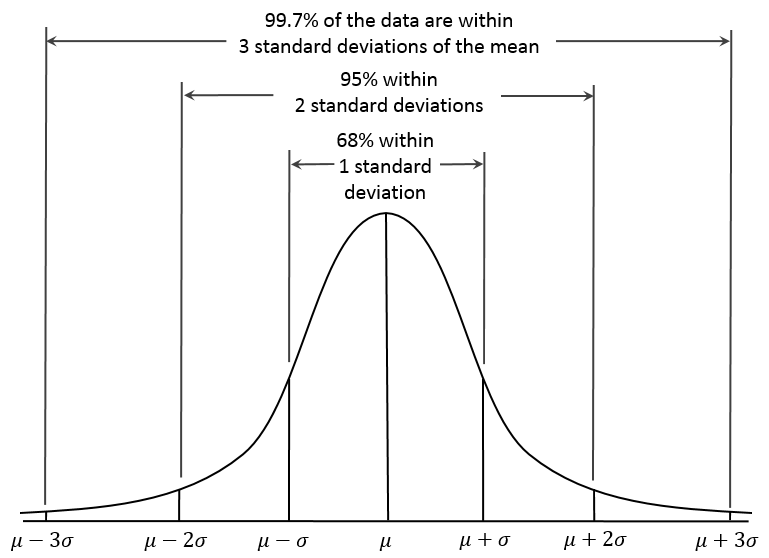
\includegraphics[width=0.8\textwidth]{figures/normal_pdf.png}
\end{figure}
\end{frame}

\begin{frame}{ The Normal Distribution}
\begin{itemize}
    \item Standard normal distribution $Z$: a normal distribution with $\mu=0$ and $\sigma=1$.
    \item We use z-tables to find the areas under the curve for $Z$.
        \begin{itemize}
            \item Given $z_0$, look for $\pr(Z\leq z_0)$.
            \item Given $p_0$, look for $z_0$ such that $\pr(Z \leq z_0) = p_0$.
        \end{itemize}
    \item If $X$ is a normal with mean $\mu$ and standard deviation $\sigma$, then
        $$\frac{X-\mu}{\sigma} \sim \mathcal{N}(0,1).$$ 
\end{itemize}
\end{frame}

%-------------------
\begin{frame}{The Central Limit Theorem (CLT)}
    Suppose $X_1,X_2,\dots,X_n$ are sampled independently from a population with mean $\mu$ and 
    standard deviation $\sigma$. Let $\bar X$ be the sample mean, 
    $$\bar X = \frac{1}{n} \sum_{i=1}^n X_i.$$
    Then,
    \begin{itemize}
        \item  $\mu_{\bar X}= \E(\bar X) = \mu$,
        \item $\sigma_{\bar X} =\sd(\bar X) =  \frac{\sigma}{\sqrt{n}}$,
        \item  If $n$ is sufficiently large ($n\geq 30$), then $\bar X$ is approximately normal.
        \item (Not by CLT) If population is normal, then $\bar X$ is normal for any $n\geq 0$.
    \end{itemize}

\end{frame}


%-------------------
\begin{frame}{Probability and Statistics}
\begin{center}
    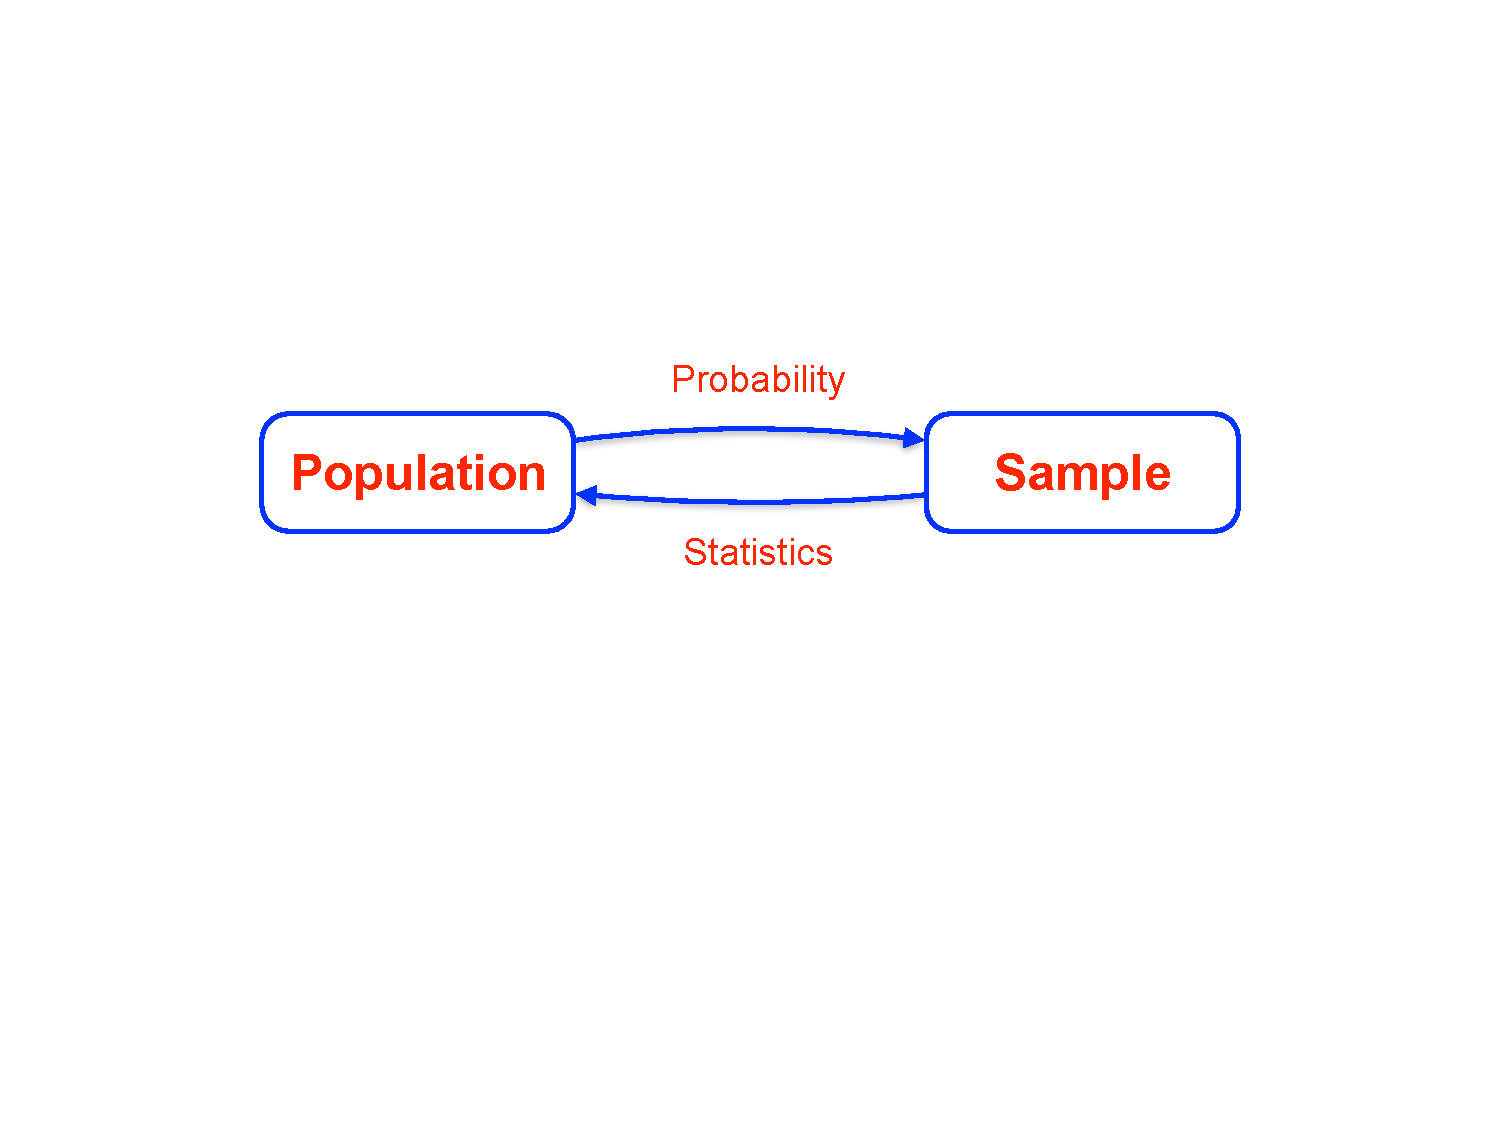
\includegraphics[width=0.8\textwidth]{figures/prob_and_stat.pdf}
\end{center}
\begin{itemize}
\item Probability: CLT, how does $\bar X$ relate to the population.
\item Statistics: estimation with confidence intervals, hypothesis testing.
\end{itemize}
\end{frame}

%-------------------
\begin{frame}{Overview of Estimation and Hypothesis Testing}
    \begin{center} \begin{tabular}{ |C|C|C|C|} \midrule
        \text{Parameter}  & \text{Estimate} & \E(\text{Estimate}) & \sd(\text{Estimate})\\\midrule
        \mu & \bar X & \mu & \sigma/{\sqrt{n}}\\ \midrule
    p & \h p & p & \sqrt{{ p (1- p)}/{n}} \\ \midrule
    \mu_1- \mu_2 & \bar X_1 - \bar X_2 & \mu_1-\mu_2 
        & \sqrt{\frac{\sigma_1^2}{n_1}+\frac{\sigma_2^2}{n_2}} \\ \midrule
\end{tabular} \end{center}

    \begin{itemize}
        \item A $1-\alpha$ CI for Parameter: $\text{Estimate} \pm (z_{\alpha/2})\, \sd(\text{Estimate}).$
        \item Hypothesis test $H_0$: Parameter=$\mu_0$  v.s. $H_A$: Parameter$\ne\mu_0$,
            $$ T = \frac{\text{Estimate}-\mu_0}{ \sd(\text{Estimate})},$$
            and compute p-value from there on.
    \end{itemize}

    \let\thefootnote\relax\footnotetext{\tiny{* Note: use $t_{\alpha/2,n-1}$ instead of $z_{\alpha/2}$ when necessary.}}
\end{frame}

%-------------------
\begin{frame}{CI for the Mean}
 \begin{table}
 \begin{center}
 \begin{tabular}{|M{3cm}|M{3cm}|M{3cm}|N}
 \hline
  & $\sigma \text{ known}$ & $\sigma \text{ unknown}$ \\[5pt]\hline
 $n\geq 30$ & 
$$ \bar X \pm z_{\alpha/2} \frac{\sigma}{\sqrt{n}}$$ & 
$$ \bar X \pm z_{\alpha/2} \frac{S}{\sqrt{n}}$$  \\[20pt] \hline
 $n< 30$, pop. is normal &  
$$ \bar X \pm z_{\alpha/2} \frac{\sigma}{\sqrt{n}} $$& 
$$ \bar X \pm \textcolor{red}{t_{\alpha/2,n-1}} \frac{S}{\sqrt{n}}$$  \\ [20pt]\hline
$n< 30$, pop. isn't normal & 
 N.A. & N.A. \\ \hline
 \end{tabular}
 \end{center}
 \end{table}
\end{frame}

%-------------------
\begin{frame}{Hypothesis Test for the Mean}
\begin{itemize}
    \item $H_0: \mu = \mu_0, \quad H_A: \mu \ne \mu_0$.
    \item Test statistic:
            $$\TS = \frac{\bar X - \mu_0 }{S/\sqrt{n}}.$$
    \item p-value: given the observed test staistic \ts,
        $$\text{p-value}=\pr(|t_{n-1}| \geq |\ts|),$$
        where $t_{n-1}$ is a t-distribution with df$=n-1$.
    \item Given significance level $\alpha$, 
        \begin{itemize}
            \item Reject $H_0$ if p-value $\leq \alpha$.
            \item Equivalently, reject $H_0$ if observe test statistic \ts\ such that
                $$t \not\in (-t_{\alpha/2,n-1}, t_{\alpha/2,n-1}).$$
        \end{itemize}
\end{itemize}
%When $H_0$ is rejected, we say that the result is statistically significant at level $\alpha$. 
\end{frame}


%-------------------
\begin{frame}{CI for the Proportion}
\begin{itemize}
\item Use $\sqrt{\frac{\h p(1-\h p)}{n}}$ as an approximation of $\sigma_{\h p} = \sqrt{\frac{p(1-p)}{n}}$. 
\item A $1-\alpha$ confidence interval for population proportion $p$ is 
\[
    \h p \pm z_{\alpha/2} \sqrt{\frac{\h p(1-\h p)}{n}}.
\]
\end{itemize}
\end{frame}


%-------------------
\begin{frame}{CI for the Difference of Means}
%    When $n_1\geq30$ and $n_2 \geq 30$,
\begin{itemize}
\item Use $\sqrt{\frac{S_1^2}{n_1} + \frac{S_2^2}{n_2} }$ as an approximation of $\sigma_{\bar X_1-\bar X_2}=\sqrt{\frac{\sigma_1^2}{n_1} + \frac{\sigma_2^2}{n_2} }$.
    \item The $1-\alpha$ confidence interval for difference of population means $\mu_1 - \mu_2$ is 
    $$
    (\bar X_1 -\bar X_2) \pm z_{\alpha/2} \sqrt{\frac{S_1^2}{n_1} + \frac{S_2^2}{n_2} }.
    $$
\end{itemize}
\end{frame}

%-------------------
\begin{frame}{Hypothesis Test for the Difference of Means}
%    When $n_1\geq30$ and $n_2 \geq 30$,
    \begin{itemize}
        \item $H_0: \mu_1 = \mu_2, \quad H_A: \mu_1 \ne \mu_2$.
        \item Test statistic:
            $$\TS = \frac{\bar X_1 - \bar X_2}{\sqrt{\frac{S_1^2}{n_1} + \frac{S_2^2}{n_2} }}.$$
        \item p-value: given the observed test staistic \ts,
        $$\text{p-value}=\pr(|Z| \geq |\ts|),$$
        where $Z$ is the standard normal random variable.
    \item Given significance level $\alpha$, 
        \begin{itemize}
            \item Reject $H_0$ if p-value $\leq \alpha$.
            \item Equivalently, reject $H_0$ if observe test statistic \ts\ such that
                $$t \not\in (-z_{\alpha/2}, z_{\alpha/2}).$$
        \end{itemize}
\end{itemize}
\end{frame}


\begin{frame}{When are CI and Htest valid?}
    The sample must satisfy
    \begin{enumerate}
        \item Observations $X_1,\cdots,X_n$ are drawn randomly and independently from the population.
            \vspace{\stretch{0.3}}
        \item We can reason about the distribution of the estimate:
            \begin{itemize}
                \item $\bar X$: population is normal, or $n\geq 30$.
            \vspace{\stretch{0.1}}
                \item $\h p$: $np \geq 15$ and $n (1-p)\geq 15$.
            \vspace{\stretch{0.1}}
                \item $\bar X_1-\bar X_2$: $n_1\geq 30$ and $n_2\geq 30$.
            \end{itemize}
    \end{enumerate}
\end{frame}

\begin{frame}{Interpretations of CI and Htest}
\begin{itemize}
\item Confidence interval: $1-\alpha$ is the probability, or proportion of the time, that a interval constructed by this procedure would cover true parameter. 
\item Hypothesis test: $\alpha$ is the probability, or proportion of the time, that a test of this kind would reject $H_0$ when $H_0$ is true.
\item Caution: there is nothing random about the true parameter or null hypothesis!
\end{itemize}
\end{frame}



\ignore{
%-------------------
\begin{frame}{Time Series Plot}
\begin{figure}
    \caption{}
    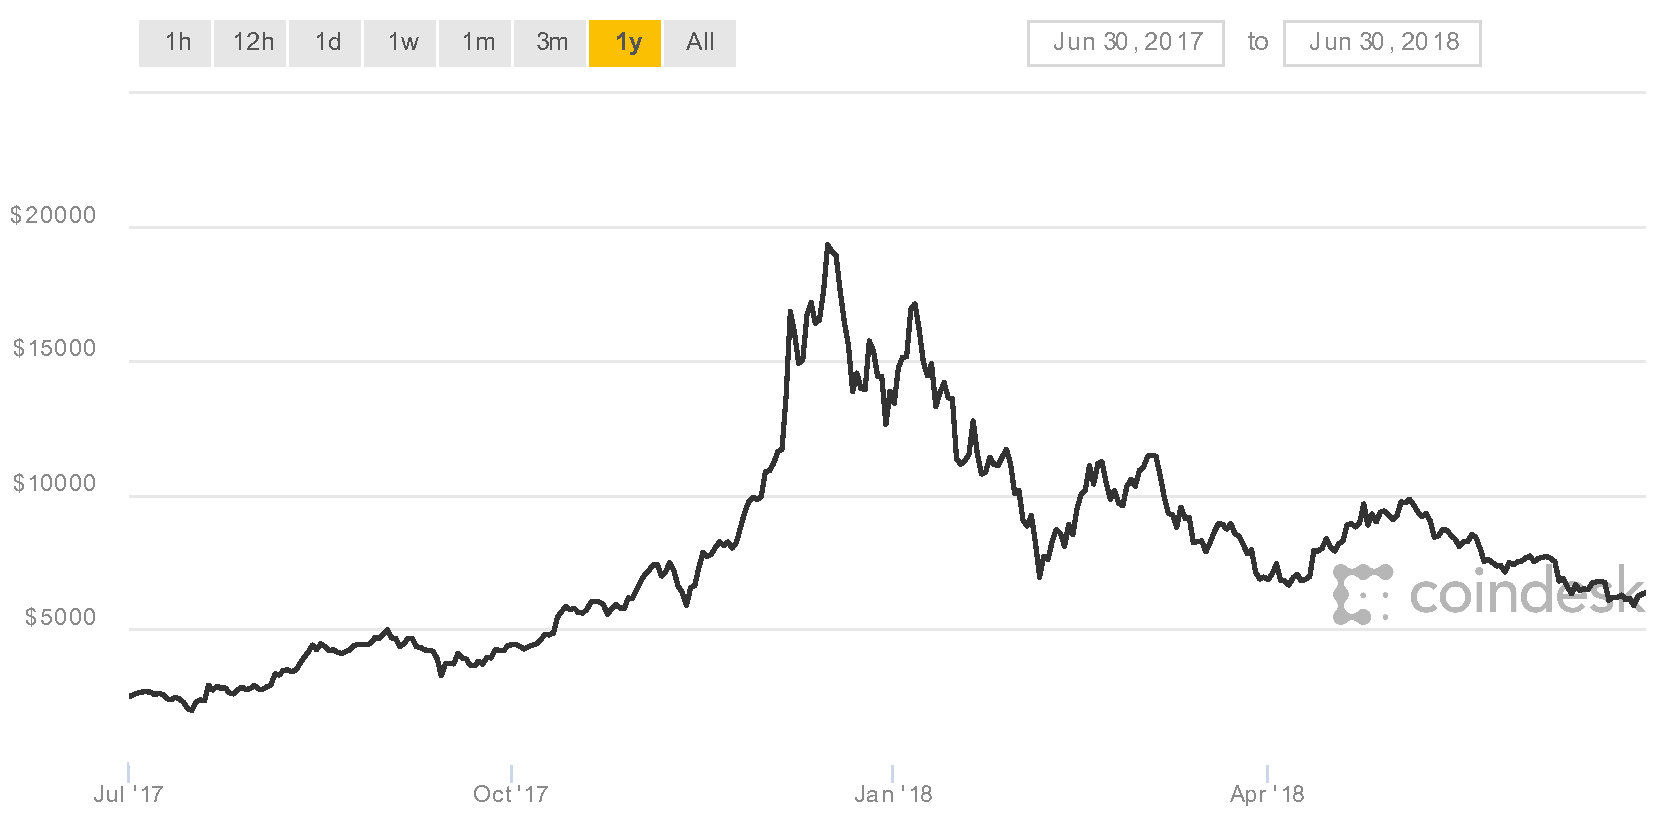
\includegraphics[width=1\textwidth]{figures/coindesk-bpi-chart}
\end{figure}
\let\thefootnote\relax\footnotetext{\tiny{* Plot from Coindesk.com}}
\end{frame}

\begin{frame}{}
\begin{itemize}
\item 
\end{itemize}
\end{frame}

\vspace{\stretch{0.5}}

\begin{block}{}
\end{block}


}

\end{document}


